% =====================================================================
%  IELTS Academic Mock Pack -- Two Mock Tests (Writing & Speaking)
%  Theme: data science and multi-agent negotiation
%  Compile with: pdflatex ielts_mock_tests.tex   (run twice for page refs)
% =====================================================================
\documentclass[10pt,a4paper]{article}

% ---------- Page & fonts ---------------------------------------------
\usepackage[a4paper,top=16mm,bottom=16mm,left=15mm,right=15mm,
            headheight=14pt,headsep=5mm,footskip=8mm]{geometry}
\usepackage[T1]{fontenc}
\usepackage[utf8]{inputenc}
\usepackage{libertine}          % Linux Libertine body, Biolinum sans
\usepackage[scaled=0.95]{roboto}% alternative sans (not default)
\renewcommand{\familydefault}{\rmdefault}
\usepackage{microtype}
\usepackage{fontawesome5}

% ---------- Graphics & boxes -----------------------------------------
\usepackage[dvipsnames,table]{xcolor}
\usepackage{tikz}
\usetikzlibrary{calc,positioning,shapes.geometric,plotmarks}
\usepackage{tcolorbox}
\tcbuselibrary{skins,breakable}
\usepackage{enumitem}
\usepackage{multicol}
\usepackage{tabularx}
\usepackage{booktabs}
\usepackage{array}
\usepackage{fancyhdr}
\usepackage{lastpage}
\usepackage{amssymb}

% ---------- Palette --------------------------------------------------
\definecolor{navy}{HTML}{16324F}
\definecolor{teal}{HTML}{127C82}
\definecolor{coral}{HTML}{E0704A}
\definecolor{gold}{HTML}{E3A72F}
\definecolor{plum}{HTML}{7A4E8C}
\definecolor{ink}{HTML}{22272E}
\definecolor{mist}{HTML}{EEF3F7}
\definecolor{sand}{HTML}{FBF5EA}
\definecolor{rule}{HTML}{C9D3DD}
\color{ink}

% ---------- Header / footer ------------------------------------------
\pagestyle{fancy}
\fancyhf{}
\renewcommand{\headrulewidth}{0pt}
\fancyhead[L]{\sffamily\footnotesize\color{navy!70}\textbf{IELTS Academic} \,·\, Mock Pack}
\fancyhead[R]{\sffamily\footnotesize\color{navy!70}Writing \& Speaking \,·\, Band 7--9 Practice}
\fancyfoot[L]{\sffamily\scriptsize\color{navy!55}Theme: Data Science \& Multi-Agent Negotiation}
\fancyfoot[R]{\sffamily\scriptsize\color{navy!55}Page \thepage\ of \pageref{LastPage}}

\setlength{\parindent}{0pt}
\setlength{\parskip}{3pt}
\setlist{nosep,leftmargin=*}
\raggedcolumns

% ---------- Components -----------------------------------------------
% Big title banner for each mock test
\newcommand{\mockbanner}[3]{%
  \begin{tcolorbox}[enhanced,colback=navy,colframe=navy,arc=3mm,
      left=6mm,right=6mm,top=3.2mm,bottom=3.2mm,boxrule=0pt,
      overlay={\begin{tcbclipinterior}\fill[#3] ([xshift=-40mm]frame.north east) rectangle (frame.south east);\end{tcbclipinterior}
               \node[font=\sffamily\bfseries\fontsize{30}{30}\selectfont,text=white]
                 at ([xshift=-20mm]frame.east) {#1};}]
    {\sffamily\color{white!75}\small\MakeUppercase{Mock Test}\,\,\faClipboardList}\\[1pt]
    {\sffamily\bfseries\color{white}\Large #2}\\[1pt]
    {\sffamily\color{white!80}\footnotesize Academic Module \,·\, Writing (60 min) \,·\, Speaking (11--14 min)}
  \end{tcolorbox}}

% Section heading chip
\newcommand{\sect}[3]{%
  \par\smallskip
  \begin{tikzpicture}[baseline=(t.base)]
    \node[fill=#1,text=white,rounded corners=1.6mm,inner xsep=2.4mm,inner ysep=1.3mm,
          font=\sffamily\bfseries\small] (t) {#2\;\;#3};
  \end{tikzpicture}\hspace{2mm}{\color{#1!60}\leaders\hrule height 0.6pt\hfill\kern0pt}\par\smallskip}

% Task box
\newtcolorbox{taskbox}[2][]{enhanced,colback=mist,colframe=#2,boxrule=0.6pt,
  leftrule=3pt,arc=2mm,left=3mm,right=3mm,top=2mm,bottom=2mm,
  fontupper=\small,#1}

% Instruction line
\newcommand{\instr}[1]{{\sffamily\footnotesize\color{navy!80}#1}\par}

% Cue card
\newtcolorbox{cuecard}[1][]{enhanced,colback=sand,colframe=gold,boxrule=0.8pt,
  arc=2mm,left=3mm,right=3mm,top=2mm,bottom=2mm,fontupper=\small,
  borderline={0.4pt}{1.2mm}{gold!60,dashed},#1}

% Tip box
\newtcolorbox{tipbox}[2][]{enhanced,colback=white,colframe=#2,boxrule=0.6pt,
  arc=2mm,left=2.5mm,right=2.5mm,top=1.5mm,bottom=1.5mm,fontupper=\footnotesize,
  title={\sffamily\bfseries\footnotesize #1},coltitle=white,colbacktitle=#2,
  attach boxed title to top left={xshift=3mm,yshift=-2mm},
  boxed title style={arc=1mm,boxrule=0pt}}

\DeclareRobustCommand{\qnum}[2]{\tikz[baseline=-0.6ex]\node[circle,fill=#1,text=white,
  inner sep=0pt,minimum size=4mm,font=\sffamily\bfseries\scriptsize]{#2};}

\newcommand{\cbox}{\raisebox{-0.2ex}{\tikz\draw[navy,line width=0.6pt,rounded corners=0.6pt] (0,0) rectangle (2.6mm,2.6mm);}}

% =====================================================================
\begin{document}
% =====================================================================

% ------------------------------ PAGE 1 -------------------------------
\mockbanner{01}{Automated Negotiation}{coral}

\sect{coral}{\faChartBar}{WRITING TASK 1 \,·\, 20 minutes \,·\, at least 150 words}

\begin{taskbox}{coral}
\instr{You should spend about 20 minutes on this task.}
The bar chart below shows the percentage of automated business negotiations that ended in an
agreement, by the type of software agent used, in \textbf{2018} and \textbf{2024}.

\textit{Summarise the information by selecting and reporting the main features, and make
comparisons where relevant.}
\end{taskbox}

\begin{center}
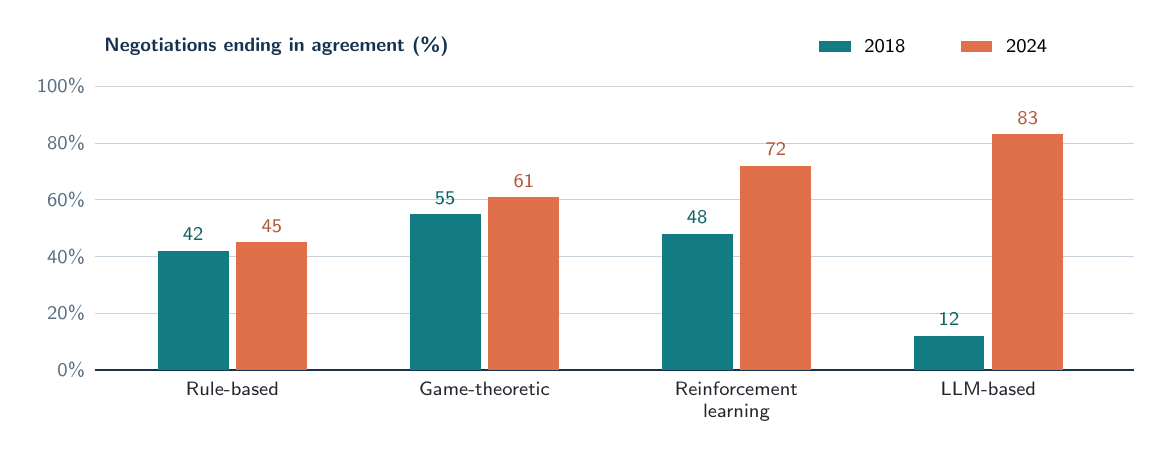
\begin{tikzpicture}[x=1mm,y=0.36mm,font=\sffamily\scriptsize]
  % grid & axes
  \foreach \v in {0,20,40,60,80,100}{
    \draw[rule,line width=0.3pt] (0,\v) -- (132,\v);
    \node[left,text=navy!70] at (0,\v) {\v\%};}
  \draw[navy,line width=0.6pt] (0,0) -- (132,0);
  % data: {label}{2018}{2024}{x}
  \foreach \lab/\a/\b/\x in {Rule-based/42/45/8,Game-theoretic/55/61/40,
                             Reinforcement\\learning/48/72/72,LLM-based/12/83/104}{
    \fill[teal]  (\x,0) rectangle ++(9,\a);
    \fill[coral] (\x+10,0) rectangle ++(9,\b);
    \node[above,text=teal!80!black]  at (\x+4.5,\a) {\a};
    \node[above,text=coral!80!black] at (\x+14.5,\b) {\b};
    \node[below,align=center,text=ink,font=\sffamily\scriptsize] at (\x+9.5,-1) {\lab};
  }
  % legend
  \fill[teal]  (92,112) rectangle ++(4,4); \node[right] at (96.5,114) {2018};
  \fill[coral] (110,112) rectangle ++(4,4); \node[right] at (114.5,114) {2024};
  \node[anchor=west,font=\sffamily\bfseries\scriptsize,text=navy] at (0,114)
      {Negotiations ending in agreement (\%)};
\end{tikzpicture}
\end{center}

\sect{coral}{\faPenNib}{WRITING TASK 2 \,·\, 40 minutes \,·\, at least 250 words}

\begin{taskbox}{coral}
\instr{You should spend about 40 minutes on this task. Write about the following topic:}
\textbf{In many industries, negotiations that were once carried out by people are now handled by
computer programs acting on their behalf.}

\textit{Do the advantages of this development outweigh the disadvantages?}

\instr{Give reasons for your answer and include any relevant examples from your own knowledge or experience.}
\end{taskbox}

\sect{teal}{\faMicrophone}{SPEAKING \,·\, Parts 1--3}

\begin{multicols}{2}
\textbf{\sffamily\small\color{teal}Part 1 \,--\, Introduction \& interview} {\footnotesize(4--5 min)}\par
\textit{\footnotesize Topic: Studies \& teamwork}
\begin{enumerate}[before=\raggedright,label=\qnum{teal}{\arabic*},leftmargin=6mm,itemsep=1.5pt,font=\small]\small
  \item What subject are you studying at the moment, and why did you choose it?
  \item Do you prefer working on projects alone or in a team? Why?
  \item How often do you have to make compromises with classmates or colleagues?
  \item Is it easy for you to say ``no'' to other people's requests?
\end{enumerate}

\columnbreak
\textbf{\sffamily\small\color{teal}Part 2 \,--\, Long turn} {\footnotesize(1 min prep + 2 min)}\par
\begin{cuecard}
\textbf{Describe a time when you had to negotiate to reach an agreement with someone.}\par\smallskip
You should say:
\begin{itemize}[label=\textcolor{gold}{\faCaretRight},leftmargin=4mm]
  \item who you negotiated with
  \item what the disagreement was about
  \item how you reached an agreement
\end{itemize}
and explain how you felt about the final outcome.
\end{cuecard}
\end{multicols}

\vspace{-1mm}
\textbf{\sffamily\small\color{teal}Part 3 \,--\, Two-way discussion} {\footnotesize(4--5 min)}
\begin{multicols}{2}
\begin{enumerate}[before=\raggedright,label=\qnum{teal!70!navy}{\arabic*},leftmargin=6mm,itemsep=1.5pt]\small
  \item Why do some people find negotiating uncomfortable, while others enjoy it?
  \item Should negotiation skills be taught formally at school? Why/why not?
  \item How might cultural differences affect the way people bargain?
  \item Would you trust an AI agent to negotiate a salary or a contract for you?
  \item What could go wrong if two AI systems negotiated with each other without human oversight?
  \item In the future, which kinds of agreements do you think will always need a human touch?
\end{enumerate}
\end{multicols}

\newpage
% ------------------------------ PAGE 2 -------------------------------
\mockbanner{02}{Data Science in Higher Education}{teal}

\sect{teal}{\faChartLine}{WRITING TASK 1 \,·\, 20 minutes \,·\, at least 150 words}

\begin{taskbox}{teal}
\instr{You should spend about 20 minutes on this task.}
The line graph below shows the number of students graduating from \textbf{Master's programmes in
Data Science} in four countries between \textbf{2014} and \textbf{2024}.

\textit{Summarise the information by selecting and reporting the main features, and make
comparisons where relevant.}
\end{taskbox}

\begin{center}
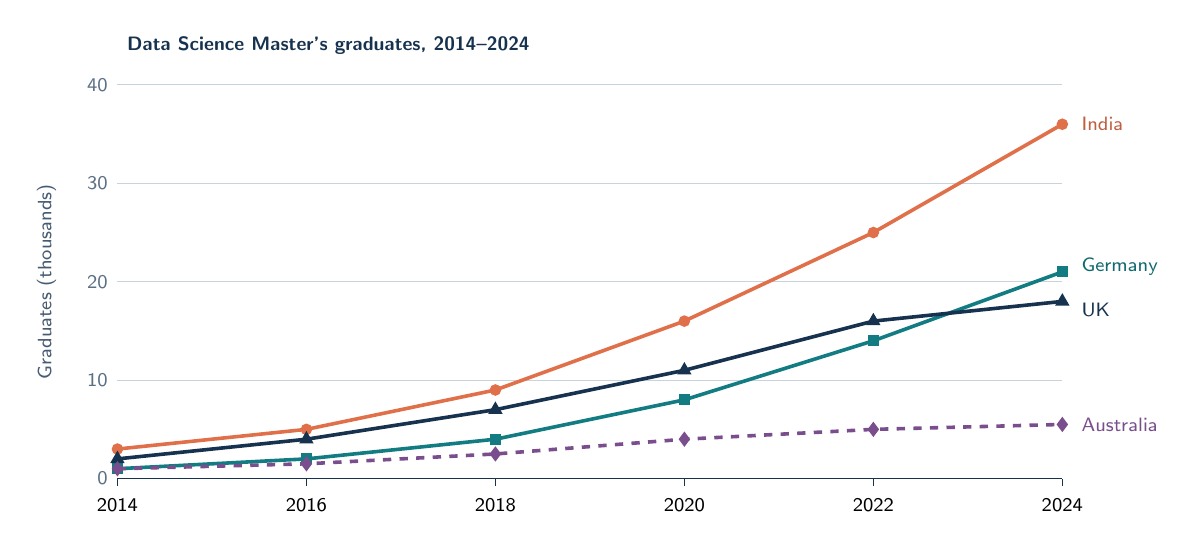
\begin{tikzpicture}[x=12mm,y=1.25mm,font=\sffamily\scriptsize]
  % grid
  \foreach \v in {0,10,20,30,40}{
    \draw[rule,line width=0.3pt] (0,\v) -- (10,\v);
    \node[left,text=navy!70] at (0,\v) {\v};}
  \foreach \yr [count=\i from 0] in {2014,2016,2018,2020,2022,2024}{
    \draw[navy,line width=0.5pt] (2*\i,0) -- ++(0,-0.8);
    \node[below=1pt] at (2*\i,-0.8) {\yr};}
  \draw[navy,line width=0.6pt] (0,0) -- (10,0);
  \node[rotate=90,text=navy!80] at (-0.75,20) {Graduates (thousands)};
  % series
  \draw[coral,line width=1.3pt] plot[mark=*,mark size=1.4pt]
     coordinates {(0,3)(2,5)(4,9)(6,16)(8,25)(10,36)};
  \draw[teal,line width=1.3pt] plot[mark=square*,mark size=1.3pt]
     coordinates {(0,1)(2,2)(4,4)(6,8)(8,14)(10,21)};
  \draw[navy,line width=1.3pt] plot[mark=triangle*,mark size=1.7pt]
     coordinates {(0,2)(2,4)(4,7)(6,11)(8,16)(10,18)};
  \draw[plum,line width=1.3pt,dashed] plot[mark=diamond*,mark size=1.7pt,mark options={solid}]
     coordinates {(0,1)(2,1.5)(4,2.5)(6,4)(8,5)(10,5.5)};
  % end labels
  \node[right,text=coral!85!black] at (10.1,36) {India};
  \node[right,text=teal!85!black]  at (10.1,21.5) {Germany};
  \node[right,text=navy]           at (10.1,17.2) {UK};
  \node[right,text=plum]           at (10.1,5.5) {Australia};
  \node[anchor=west,font=\sffamily\bfseries\scriptsize,text=navy] at (0,44)
      {Data Science Master's graduates, 2014--2024};
\end{tikzpicture}
\end{center}

\sect{teal}{\faPenNib}{WRITING TASK 2 \,·\, 40 minutes \,·\, at least 250 words}

\begin{taskbox}{teal}
\instr{You should spend about 40 minutes on this task. Write about the following topic:}
\textbf{Some people believe that universities should concentrate on practical, job-ready skills such
as programming and data analysis. Others argue that universities should prioritise deep theoretical
knowledge.}

\textit{Discuss both these views and give your own opinion.}

\instr{Give reasons for your answer and include any relevant examples from your own knowledge or experience.}
\end{taskbox}

\sect{coral}{\faMicrophone}{SPEAKING \,·\, Parts 1--3}

\begin{multicols}{2}
\textbf{\sffamily\small\color{coral}Part 1 \,--\, Introduction \& interview} {\footnotesize(4--5 min)}\par
\textit{\footnotesize Topic: Technology \& numbers}
\begin{enumerate}[before=\raggedright,label=\qnum{coral}{\arabic*},leftmargin=6mm,itemsep=1.5pt]\small
  \item Which app or website do you use most often each day?
  \item Were you good at mathematics when you were a child?
  \item Do you enjoy reading charts and statistics in the news? Why?
  \item Has technology made your studies easier or more stressful?
\end{enumerate}

\columnbreak
\textbf{\sffamily\small\color{coral}Part 2 \,--\, Long turn} {\footnotesize(1 min prep + 2 min)}\par
\begin{cuecard}
\textbf{Describe a piece of research or a project you are proud of.}\par\smallskip
You should say:
\begin{itemize}[label=\textcolor{gold}{\faCaretRight},leftmargin=4mm]
  \item what the project was about
  \item who you worked with
  \item what difficulties you faced
\end{itemize}
and explain why you are proud of it.
\end{cuecard}
\end{multicols}

\vspace{-1mm}
\textbf{\sffamily\small\color{coral}Part 3 \,--\, Two-way discussion} {\footnotesize(4--5 min)}
\begin{multicols}{2}
\begin{enumerate}[before=\raggedright,label=\qnum{coral!70!navy}{\arabic*},leftmargin=6mm,itemsep=1.5pt]\small
  \item Why do you think data-related jobs have become so popular recently?
  \item Should governments fund pure research that has no obvious practical use?
  \item How can ordinary people tell whether a statistic in the media is reliable?
  \item Is it fair that companies collect so much personal data from their users?
  \item Will artificial intelligence make university degrees less valuable?
  \item How should researchers from different countries share data and credit fairly?
\end{enumerate}
\end{multicols}

\newpage
% ------------------------------ PAGE 3 -------------------------------
\begin{tcolorbox}[enhanced,colback=navy,colframe=navy,arc=3mm,boxrule=0pt,
    left=6mm,right=6mm,top=3.2mm,bottom=3.2mm,
    overlay={\begin{tcbclipinterior}\fill[gold] ([xshift=-40mm]frame.north east) rectangle (frame.south east);\end{tcbclipinterior}
             \node[text=white,font=\fontsize{26}{26}\selectfont] at ([xshift=-20mm]frame.east) {\faToolbox};}]
  {\sffamily\color{white!75}\small EXAMINER'S TOOLKIT\,\,\faLightbulb}\\[1pt]
  {\sffamily\bfseries\color{white}\Large Band Criteria, Model Language \& Self-Check}\\[1pt]
  {\sffamily\color{white!80}\footnotesize Use this page after each mock to mark yourself honestly.}
\end{tcolorbox}

\sect{navy}{\faBalanceScale}{HOW YOU ARE MARKED \,·\, Writing (each criterion = 25\%)}

{\small
\renewcommand{\arraystretch}{1.25}
\begin{tabularx}{\linewidth}{>{\raggedright\arraybackslash\leavevmode\color{navy}\sffamily\bfseries}p{34mm} >{\raggedright\arraybackslash}X >{\raggedright\arraybackslash}X}
\toprule
\rowcolor{mist}Criterion & \sffamily\bfseries Band 7 looks like\ldots & \sffamily\bfseries Band 8--9 looks like\ldots\\
\midrule
Task Achievement / Response & Clear overview (T1); position is clear throughout (T2) & Well-selected key features; fully developed, extended ideas\\
Coherence \& Cohesion & Logical paragraphing; a range of linkers, occasionally overused & Cohesion is ``invisible''; paragraphing is skilful\\
Lexical Resource & Some less common items; occasional collocation errors & Wide, precise, natural vocabulary; rare slips only\\
Grammatical Range \& Accuracy & Frequent error-free sentences; varied structures & Wide range; the majority of sentences error-free\\
\bottomrule
\end{tabularx}}

\vspace{1mm}
\begin{multicols}{2}
\begin{tipbox}[\faStar\; Model overview \,--\, Mock 1, Task 1]{coral}
\itshape Overall, every type of agent reached agreement more often in 2024 than in 2018, but the
scale of improvement varied dramatically. The most striking change was in LLM-based agents, which
rose from being by far the least successful (12\%) to the most successful (83\%), whereas
rule-based systems remained almost static at just under half.
\end{tipbox}

\begin{tipbox}[\faStar\; Model thesis \,--\, Mock 2, Task 2]{teal}
\itshape While job-ready skills undeniably help graduates enter the labour market, I would argue
that theory is what allows them to stay employable once today's tools become obsolete; therefore
the best degrees integrate the two rather than choose between them.
\end{tipbox}

\begin{tipbox}[\faStopwatch\; Timing plan]{plum}
\begin{tabular}{@{}l@{\;}l@{}}
\textbf{T1:} & 3 plan \,·\, 14 write \,·\, 3 check\\
\textbf{T2:} & 5 plan \,·\, 30 write \,·\, 5 check\\
\textbf{Speaking P2:} & jot 4--5 key words, not sentences
\end{tabular}
\end{tipbox}

\columnbreak

\begin{tipbox}[\faChartLine\; Language bank \,--\, trends \& data]{navy}
\textbf{Rise:} surge, soar, climb steadily, a sharp/threefold increase\\
\textbf{Fall:} decline, dip, plummet, a marginal decrease\\
\textbf{Stable:} plateau, level off, remain virtually unchanged\\
\textbf{Compare:} outstrip, lag behind, twice as many as, by contrast\\
\textbf{Approximate:} just under a half, roughly a third, nearly
\end{tipbox}

\begin{tipbox}[\faUsers\; Language bank \,--\, negotiation \& AI]{gold}
\textbf{Nouns:} concession, trade-off, stakeholder, consensus, leverage, deadlock, mutual gain\\
\textbf{Verbs:} bargain, compromise, mediate, reach/strike a deal, reconcile interests\\
\textbf{AI terms:} autonomous agent, algorithmic bias, accountability, transparency, human-in-the-loop\\
\textbf{Hedging:} it could be argued that, to a certain extent, arguably
\end{tipbox}

\begin{tcolorbox}[enhanced,colback=mist,colframe=navy!40,boxrule=0.5pt,arc=2mm,
    left=2.5mm,right=2.5mm,top=1.5mm,bottom=1.5mm,fontupper=\footnotesize]
{\sffamily\bfseries\color{navy}\faCheckSquare\; Self-check before you stop writing}\par\smallskip
\cbox\; T1 has a clear overview paragraph (no opinions!)\par
\cbox\; Key numbers are compared, not just listed\par
\cbox\; T2 answers \emph{every} part of the question\par
\cbox\; Each body paragraph has one main idea + example\par
\cbox\; Word count: T1 $\geq$ 150, T2 $\geq$ 250\par
\cbox\; Checked articles, plurals and subject--verb agreement
\end{tcolorbox}
\end{multicols}

\vspace{1mm}
\sect{teal}{\faComments}{SPEAKING BOOSTERS \,·\, Fluency, vocabulary \& pronunciation}

\begin{multicols}{2}
\begin{tipbox}[\faLayerGroup\; Extend every answer: A\,--\,R\,--\,E]{teal}
\textbf{A}nswer directly \,$\rightarrow$\, give a \textbf{R}eason \,$\rightarrow$\, add an \textbf{E}xample.\par\smallskip
\itshape ``I'd trust an AI agent with routine deals, \textup{(A)} because it can compare
thousands of offers without getting tired or emotional. \textup{(R)} For instance, some
energy companies already let algorithms bargain over electricity prices every few
minutes.'' \textup{(E)}
\end{tipbox}

\columnbreak
\begin{tipbox}[\faExclamationTriangle\; Five Band-6 traps to avoid]{coral}
\begin{enumerate}[label=\textbf{\arabic*.},leftmargin=4mm]
  \item Describing every number in Task 1 instead of grouping trends.
  \item Memorised openers (``Nowadays, with the development of\ldots'').
  \item Giving an opinion in Task 1 or none at all in Task 2.
  \item One-word or one-sentence answers in Speaking Part 1.
  \item Using fillers (``like'', ``you know'') instead of pausing naturally.
\end{enumerate}
\end{tipbox}
\end{multicols}

\vfill
\begin{tcolorbox}[enhanced,colback=sand,colframe=gold,boxrule=0.5pt,arc=2mm,
    left=3mm,right=3mm,top=1.5mm,bottom=1.5mm,fontupper=\footnotesize]
\textbf{\sffamily\color{navy}\faRoute\; Score tracker}\hfill
\begin{tabular}{l*{5}{c}}
 & \sffamily TA/TR & \sffamily CC & \sffamily LR & \sffamily GRA & \sffamily \textbf{Overall}\\
\sffamily Mock 1 & \rule{9mm}{0.4pt} & \rule{9mm}{0.4pt} & \rule{9mm}{0.4pt} & \rule{9mm}{0.4pt} & \rule{11mm}{0.4pt}\\[2pt]
\sffamily Mock 2 & \rule{9mm}{0.4pt} & \rule{9mm}{0.4pt} & \rule{9mm}{0.4pt} & \rule{9mm}{0.4pt} & \rule{11mm}{0.4pt}\\
\end{tabular}
\end{tcolorbox}

\end{document}
